\documentclass[a4j,11pt]{ltjsarticle}    % 文章クラスとオプション設定
%%%%%%%%%% スタイル %%%%%%%%%%%%%%%%%%%%%%%%%%%%%%%%%%%%%%%%%%%%%%%%%%%%%%%%%%%%%%%%%%%%%%%%%%%%%%

\usepackage{comment}    % 複数行コメント

% 余白の調整
\usepackage[top=30truemm,bottom=30truemm,left=20truemm,right=20truemm]{geometry}

% 数式関連
\usepackage{amsmath,amssymb,nccmath,siunitx}    % 数式
\usepackage{bm}         % ベクトルの太文字
\newcommand{\alignref}[1]{\textbf{式(\ref{#1})}}    % 数式参照
\usepackage{siunitx}

% 画像関連
\usepackage{pdfpages} % PDF
\usepackage{graphicx} % 画像

\usepackage{here}% figureの位置調整
% 表設定
\usepackage{multirow}   % 表の行の結合
\usepackage{longtable}  % ページをまたぐ長い表
\usepackage{url}

%%%%%%%%%% 本文 %%%%%%%%%%%%%%%%%%%%%%%%%%%%%%%%%%%%%%%%%%%%%%%%%%%%%%%%%%%%%%%%%%%%%%%%%%%%%%%%%

\begin{document}

% !TEX root = main.tex

%%%%%%%%%%%%%%%%%%%%%%%%%%%%%%%%%%%%%%%%%%%%%%%%%%%%%%%%%%%%%%%%%%%%%%%%%%%%%%%%%%%%%%%%%%%%%%%%

\title{制御工学 レポート課題}
\author{21121001 浅井雅史}
\date{}
\maketitle

%%%%%%%%%%%%%%%%%%%%%%%%%%%%%%%%%%%%%%%%%%%%%%%%%%%%%%%%%%%%%%%%%%%%%%%%%%%%%%%%%%%%%%%%%%%%%%%%

% \setcounter{tocdepth}{3}
% \tableofcontents
% \newpage

① つぎの伝達関数をもつシステムのインディシャル応答 (ステップ入力に対する応答) を計算せよ.

$$
a)\,\frac{s^2-5 s-12}{(s+1)(s+2)(s+3)}\quad
b)\,\frac{2 s^2+10 s-10}{(s+1)\left(s^2+2 s+10\right)}
$$

\begin{align*}
    a)\,\mathcal{L}^{-1}[\frac{s^2-5s-12}{s(s+1)(s+2)(s+3)}]
    &=\frac{3}{s+1}+\frac{1}{s+2}-\frac{2}{s+3}-\frac{2}{s} \\
    &=3e^{-t}+e^{-2t}-2e^{-3t}-2 \\
\end{align*}

\begin{align*}
    b)\,\mathcal{L}^{-1}[\frac{2s^2+10s-10}{s(s+1)(s^2+2s+10)}]
    &=\frac{2-s}{s^2+2s+10}-\frac{1}{s}+\frac{2}{s+1} \\
    &=-\frac{s+1}{(s+1)^2+3^2}+\frac{3}{(s+1)^2+3^2}-\frac{1}{s}+\frac{2}{s+1} \\
    &=-e^{-t}\cos3t+3e^{-t}\sin3t-1+2e^{-t} \\
\end{align*}
② 伝達関数の分母多項式がつぎのように与えられるとき,システムが安定か否か判別せよ.
$$
a)\,s^3+5s^2+9s+5\quad
b)\,2s^3+5s^2+6s+2
$$
表1,表2より,どちらも安定である.

\begin{table}[H]
    \centering
    \begin{tabular}{c|ccc}
        \hline
        $s^3$ & 1 & 9 & 0 \\
        $s^2$ & 5 & 5 & 0 \\
        $s^1$ & $8=-\frac{1\times 5-5\times 9}{5}$ & 0 &  \\
        $s^0$ & $5=-\frac{5\times 0-8\times 5}{8}$ & 0 &  \\ \hline
        
    \end{tabular}
    \caption{a)のラウス表}
\end{table}

\begin{table}[H]
    \centering
    \begin{tabular}{c|ccc}
        \hline
        $s^3$ & 2 & 6 & 0 \\
        $s^2$ & 5 & 2 & 0 \\
        $s^1$ & $\frac{26}{5}=-\frac{2\times 2-5\times 6}{5}$ & 0 & 0 \\
        $s^0$ & $5=-\frac{5\times 0-\frac{26}{5}\times 2}{\frac{26}{5}}$ & 0 & 0 \\ \hline
        
    \end{tabular}
    \caption{b)のラウス表}
\end{table}
③ 制御器の伝達関数$K(s)$と制御対象の伝達関数$P(s)$がつぎのように与えられるとき,
$$
K(s)=K, K>0, \quad P(s)=\frac{1}{s^3+5 s^2+11 s+15}
$$
このフィードバック制御系が安定となる$K$ の範囲を求めよ.


伝達関数を求めると,
$$
K(s)=K, K>0, \quad P(s)=\frac{1}{s^3+5 s^2+11 s+15}
$$
であるので,表3より,$0<K<40$である.

\begin{table}[H]
    \centering
    \begin{tabular}{c|ccc}
        \hline
        $s^3$ & 1 & 11 & 0 \\
        $s^2$ & 5 & $15+K$ & 0 \\
        $s^1$ & $\frac{-K+40}{5}$ & 0 & 0 \\
        $s^0$ & $K+15$ & 0 & 0 \\ \hline
        
    \end{tabular}
    \caption{ラウス表}
\end{table}
④ つぎの伝達関数のゲイン線図(ボード線図のゲインの図)を,折れ線近似を用いて描け.ただし,折れ
点の周波数とそのときのゲインのデシベル値がわかるように描くこと.
$$
\frac{10(s+10)}{s(s+1)(s+100)}
$$


$$
\frac{100(s+10)}{s(s+1)(s+100)}=\frac{100 \cdot 10(0.1 s+1)}{100 s(s+1)(0.01 s+1)}=10 \cdot \frac{1}{s} \cdot \frac{1}{s+1} \cdot \frac{1}{0.01 s+1} \cdot(0.1 s+1)
$$

\newpage

⑤つぎのシステムについて,問いに答えよ.
$$
\frac{\mathrm{d}}{\mathrm{d} t} \boldsymbol{x}(t)=\boldsymbol{A} \boldsymbol{x}(t)+\boldsymbol{b} u(t), \quad \boldsymbol{A}=\left[\begin{array}{cc}
0 & 1 \\
-3 & -4
\end{array}\right], \quad \boldsymbol{b}=\left[\begin{array}{l}
1 \\
1
\end{array}\right]
$$

a)\,逆ラプラス変換を利用して$e^{At}$を求めよ.


b)\,$\boldsymbol{x}(0)=\left[\begin{array}{ll}-1 & 1\end{array}\right]^T, u(t) \equiv 1$
としたときのシステムの解軌道$x(t)$を求めよ.


$$
\begin{aligned}
    a)\,
    \mathrm{e}^{A t} & =\mathcal{L}^{-1}\left\{(s I-A)^{-1}\right\}=\mathcal{L}^{-1}\left\{\left[\begin{array}{cc}
    s & -1 \\
    3 & s+4
    \end{array}\right]^{-1}\right\}=\mathcal{L}^{-1}\left\{\frac{1}{s^2+4 s+3}\left[\begin{array}{cc}
    s+4 & 1 \\
    -3 & s
    \end{array}\right]\right\} \\
    & =\mathcal{L}^{-1}\left\{\left[\begin{array}{cc}
    \frac{3}{2} \frac{1}{s+1}-\frac{1}{2} \frac{1}{s+3} & \frac{1}{2} \frac{1}{s+1}-\frac{1}{2} \frac{1}{s+3} \\
    -\frac{3}{2} \frac{1}{s+1}+\frac{3}{2} \frac{1}{s+3} & -\frac{1}{2} \frac{1}{s+1}+\frac{3}{2} \frac{1}{s+3}
    \end{array}\right]\right\}=\left[\begin{array}{cc}
    \frac{3}{2} \mathrm{e}^{-t}-\frac{1}{2} \mathrm{e}^{-3 t} & \frac{1}{2} \mathrm{e}^{-t}-\frac{1}{2} \mathrm{e}^{-3 t} \\
    -\frac{3}{2} \mathrm{e}^{-t}+\frac{3}{2} \mathrm{e}^{-3 t} & -\frac{1}{2} \mathrm{e}^{-t}+\frac{3}{2} \mathrm{e}^{-3 t}
    \end{array}\right]
\end{aligned}
$$


$$
\begin{aligned}
    b)\,
    & \int_0^t \mathrm{e}^{A(t-\tau)} b u(\tau) d \tau=\int_0^t\left[\begin{array}{ll}
    \frac{3}{2} \mathrm{e}^{\tau-t}-\frac{1}{2} \mathrm{e}^{3(\tau-t)} & \frac{1}{2} \mathrm{e}^{\tau-t}-\frac{1}{2} \mathrm{e}^{3(\tau-t)} \\
    -\frac{3}{2} \mathrm{e}^{\tau-t}+\frac{3}{2} \mathrm{e}^{3(\tau-t)} & -\frac{1}{2} \mathrm{e}^{\tau-t}+\frac{3}{2} \mathrm{e}^{3(\tau-t)}
    \end{array}\right]\left[\begin{array}{l}
    1 \\
    1
    \end{array}\right] d \tau \\
    & =\int_0^t\left[\begin{array}{c}
    2 \mathrm{e}^{-t} \mathrm{e}^\tau-\mathrm{e}^{-3 t} \mathrm{e}^{3 \tau} \\
    -2 \mathrm{e}^{-t} \mathrm{e}^\tau+3 \mathrm{e}^{-3 t} \mathrm{e}^{3 \tau}
    \end{array}\right] d \tau=\left[\left[\begin{array}{c}
    2 \mathrm{e}^{-t} \mathrm{e}^\tau-\mathrm{e}^{-3 t} \frac{1}{3} \mathrm{e}^{3 \tau} \\
    -2 \mathrm{e}^{-t} \mathrm{e}^\tau+\mathrm{e}^{-3 t} \mathrm{e}^{3 \tau}
    \end{array}\right]\right]_0^t \\
    & =\left[\begin{array}{c}
    2-\frac{1}{3}-\left(2 \mathrm{e}^{-t}-\frac{1}{3} \mathrm{e}^{-3 t}\right) \\
    -2+1-\left(-2 \mathrm{e}^{-t}+\mathrm{e}^{-3 t}\right)
    \end{array}\right]=\left[\begin{array}{c}
    \frac{5}{3}-2 \mathrm{e}^{-t}+\frac{1}{3} \mathrm{e}^{-3 t} \\
    -1+2 \mathrm{e}^{-t}-\mathrm{e}^{-3 t}
    \end{array}\right]
    \end{aligned}
$$
$$
\begin{aligned}
x(t) & =\mathrm{e}^{A t} x(0)+\int_0^t \mathrm{e}^{A(t-\tau)} b u(\tau) d \tau=\left[\begin{array}{cc}
\frac{3}{2} \mathrm{e}^{-t}-\frac{1}{2} \mathrm{e}^{-3 t} & \frac{1}{2} \mathrm{e}^{-t}-\frac{1}{2} \mathrm{e}^{-3 t} \\
-\frac{3}{2} \mathrm{e}^{-t}+\frac{3}{2} \mathrm{e}^{-3 t} & -\frac{1}{2} \mathrm{e}^{-t}+\frac{3}{2} \mathrm{e}^{-3 t}
\end{array}\right]\left[\begin{array}{l}
1 \\
1
\end{array}\right]+\left[\begin{array}{c}
\frac{5}{3}-2 \mathrm{e}^{-t}+\frac{1}{3} \mathrm{e}^{-3 t} \\
-1+2 \mathrm{e}^{-t}-\mathrm{e}^{-3 t}
\end{array}\right] \\
& =\left[\begin{array}{c}
2 \mathrm{e}^{-t}-\mathrm{e}^{-3 t} \\
-2 \mathrm{e}^{-t}+3 \mathrm{e}^{-3 t}
\end{array}\right]+\left[\begin{array}{l}
\frac{5}{3}-2 \mathrm{e}^{-t}+\frac{1}{3} \mathrm{e}^{-3 t} \\
-1+2 \mathrm{e}^{-t}-\mathrm{e}^{-3 t}
\end{array}\right]=\left[\begin{array}{c}
\frac{5}{3}-\frac{2}{3} \mathrm{e}^{-3 t} \\
-1+2 \mathrm{e}^{-3 t}
\end{array}\right]
\end{aligned}
$$

\newpage

⑥ つぎの開ループ伝達関数をもつ制御系のゲイン余裕を$40\,\mathrm{dB}$とする
$K$の値を示せ.
$$
G(s)=\frac{K}{(2s+1)(s+1)(s+3)}
$$


$$
G(j \omega)=\frac{K}{(2 j \omega+1)(j \omega+1)(j \omega+3)}=\frac{K}{\left(-2 \omega^2+3 j \omega+1\right)(j \omega+3)}=\frac{K}{3\left(1-3 \omega^2\right)+j \omega\left(10-2 \omega^2\right)}
$$
これより,位相交差周波数は$\omega_{pc}=\sqrt[]{5}$である.子の周波数の時のゲインの逆数の大きさがゲイン余裕であり,
$$
GM=40 \log _{10}\left|\frac{1}{G\left(j \omega_{p c}\right)}\right|=40 \log _{10} \frac{42}{K} \mathrm{~dB}
$$
と求められる.これが$40\,\mathrm{dB}$となる$K$は,$\frac{42}{K}=10^1$より,$K=\frac{42}{10}=\frac{21}{5}$である.
\newpage

⑦ 次の図の制御系について以下の問いに答えよ.
\begin{figure}[H]
    \centering
    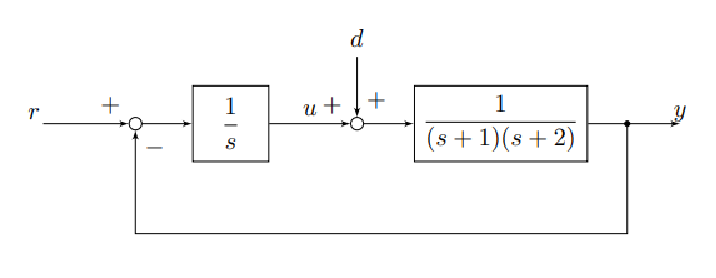
\includegraphics[scale=0.75]{figure1.pdf}
\end{figure}

a)\,$d(t)\equiv 0$としたときの目標値$r(t)$に対する定常位置偏差を求めよ.

b)\,$r(t)\equiv 0$であるとする.ランプ外乱$d(t)=t$を加えた時の$y(t)$の定常値を求めよ.

%%%%%%%%%% 参考文献 %%%%%%%%%%%%%%%%%%%%%%%%%%%%%%%%%%%%%%%%%%%%%%%%%%%%%%%%%%%%%%%%%%%%%%%%%%%%%%

% \input{ref.tex}

\end{document}